\documentclass[a4paper,12pt,norsk]{article}
\usepackage[utf8]{inputenc}
\usepackage{textcomp}
\usepackage[T1]{fontenc}
\usepackage[norsk]{babel}
\usepackage{amsmath}
\usepackage{amsfonts}
\usepackage{amsthm}
\usepackage[colorlinks]{hyperref}
\usepackage{listings}
\usepackage{graphicx}
\usepackage{caption}
\usepackage{varioref}
\usepackage{gensymb}
\usepackage{cancel}
\lstset{
	tabsize=4,
	rulecolor=,
	language=python,
        basicstyle=\scriptsize,
        upquote=true,
        aboveskip={1.5\baselineskip},
        columns=fixed,
	numbers=left,
        showstringspaces=false,
        extendedchars=true,
        breaklines=true,
        prebreak = \raisebox{0ex}[0ex][0ex]{\ensuremath{\hookleftarrow}},
        frame=single,
        showtabs=false,
        showspaces=false,
        showstringspaces=false,
        identifierstyle=\ttfamily,
        keywordstyle=\color[rgb]{0,0,1},
        commentstyle=\color[rgb]{0.133,0.545,0.133},
        stringstyle=\color[rgb]{0.627,0.126,0.941}
        }

\title{MAT 1110 Obligatorisk oppgave 2}
\author{Kenneth Ramos Eikrehagen}
\begin{document}
\maketitle
\tableofcontents
\section{Oppgave 1}
\subsection{a)}
Jeg har fått oppgitt at 50\% av A går til B, 50\% av B går ti C og 50\% av C går til A. Jeg setter opp en matrise M der første søyle representerer de kulene som startet i A, midterste søyle er de som startet i B og siste søyle er de som startet i C. 

\begin{align*}
M =
\begin{pmatrix}
\frac{1}{2} & 0 & \frac{1}{2} \\
\frac{1}{2} & \frac{1}{2} & 0 \\
0 & \frac{1}{2} & \frac{1}{2}
\end{pmatrix}
\sim
\begin{pmatrix}
1 & 0 & 1 \\
1 & 1 & 0 \\
0 & 1 & 1
\end{pmatrix}
\end{align*}

Siden jeg skal skrive M som $\frac{1}{2}M$ kan jeg bruke at 
\begin{align*}
M =
\begin{pmatrix}
1 & 0 & 1 \\
1 & 1 & 0 \\
0 & 1 & 1
\end{pmatrix}
\end{align*}

Siden 
\begin{align*}
\bold{x}_n = 
\left({\begin{array}{cc} x_n\\ y_n\\ z_n  \end{array}}\right)
\end{align*}

Så vil vektoren $\bold{x}_{n+1} = \frac{1}{2}M\bold{x}_n$ gi neste tidsenhet. 

\subsection{b)}
Denne løste jeg ved hjelp av matlab.\\
\begin{figure}[h!]
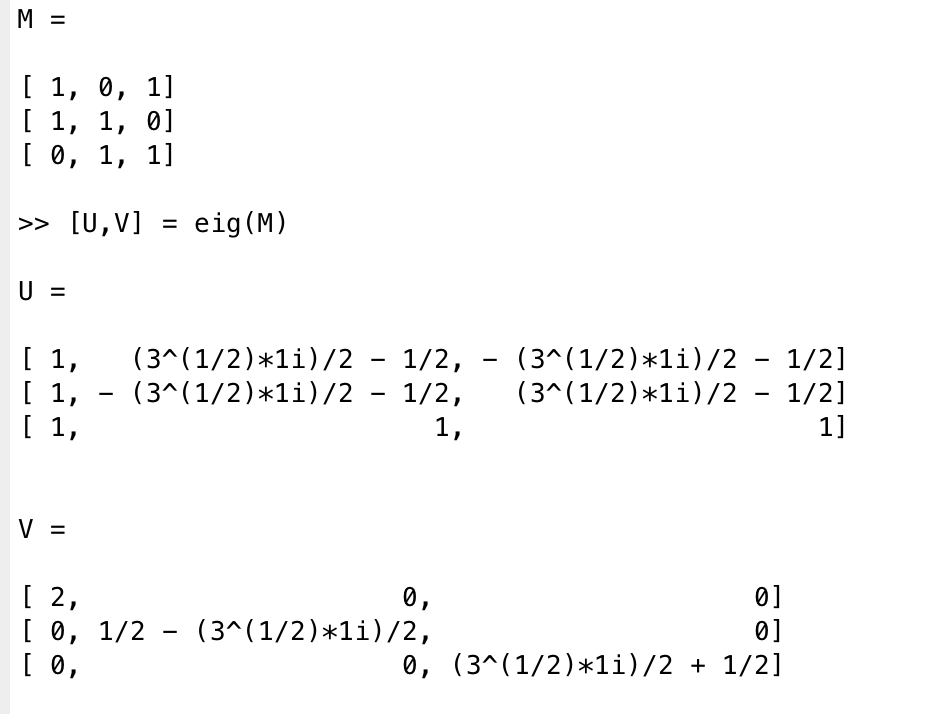
\includegraphics[width = 1\textwidth]{11b.png} 
\caption{u = egen vektorene, v = egenverdiene}
\label{1b}
\end{figure} 

Som vi ser på figur \vref{1b} er egen vektorene: 
\begin{align*}
\bold{v}_1 = \left({\begin{array}{cc} 1\\ 1\\ 1  \end{array}}\right) \textbf{, }
\bold{v}_2 = \left({\begin{array}{cc} -\frac{1-\sqrt{3}i}{2}\\ -\frac{1+\sqrt{3}i}{2}\\ 1  \end{array}}\right)\textbf{, } 
\bold{v}_3 = \left({\begin{array}{cc} -\frac{1+\sqrt{3}i}{2}\\ -\frac{1-\sqrt{3}i}{2}\\ 1  \end{array}}\right)
\end{align*}
Med tilhørende egenverdier:
\begin{align*}
\lambda_1 = 1 \textbf{, } \lambda_2 = \frac{1-\sqrt{3}i}{2} \textbf{, } \lambda_3 = \frac{1+\sqrt{3}i}{2} 
\end{align*}

\subsection{c)}
Fordi at $\bold{v}_1 \textbf{, }\bold{v}_2\textbf{, }\bold{v}_3$ er forskjellige vet jeg at disse lager en basis. Start fasen $x_0$ kan derfor skrives som en lineærkombinasjon av egenvektorene: 
$$x_0 = c_1\bold{v}_1 + c_2\bold{v}_2 + c_3\bold{v}_3 $$
Hvis vi lar kulene bare flytte seg fritt vet jeg at jeg da kan uttrykke $x_m = M^mx_0$ (bruker m siden n er allerede brukt) Ganger jeg nå $M^m$ på begge sider av $x_0$ får jeg :

\begin{align*}
x_m &= M^mx_0 = c_1M^m\bold{v}_1 + c_2M^m\bold{v}_2 + c_3M^m\bold{v}_3\\
&= c_1\lambda_1^m\bold{v}_1 + c_2\lambda_2^m\bold{v}_2 + c_3\lambda_3^m\bold{v}_3\\
& = c_1\bold{v}_1 + c_2\Big(\frac{1-\sqrt{3}i}{2}\Big)^m\bold{v}_2 + c_3\Big(\frac{1+\sqrt{3}i}{2}\Big)^m\bold{v}_3\\
\end{align*}
Jeg må nå finne hva $c_1$, $c_2$, $c_3$ er. Dette kan jeg gjøre ved å sette inn verdien 
\begin{align*}
x_0 = 
\begin{pmatrix} 100\\ 0\\ 0 \end{pmatrix}
\end{align*} og løse:  
 \begin{align*}
 c_1 \left({\begin{array}{cc} 1\\ 1\\ 1  \end{array}}\right) - 
 c_2 \left({\begin{array}{cc} -\frac{1-\sqrt{3}i}{2}\\ -\frac{1+\sqrt{3}i}{2}\\ 1  \end{array}}\right) -
 c_3 \left({\begin{array}{cc} -\frac{1+\sqrt{3}i}{2}\\ -\frac{1-\sqrt{3}i}{2}\\ 1  \end{array}}\right) = 
 \begin{pmatrix} 100\\ 0\\ 0 \end{pmatrix}\\
 \end{align*}
 Dette er ekvivalent med ligningssystemet:
 \begin{align*}
 c_1 + \Big(\frac{1-\sqrt{3}i}{2}\Big)c_2 + \Big(\frac{1+\sqrt{3}i}{2}\Big)c_3 &= 100\\
 c_1 + \Big(\frac{1+\sqrt{3}i}{2}\Big)c_2 + \Big(\frac{1-\sqrt{3}i}{2}\Big)c_3 &= 0\\
 c_1 + c_2 + c_3 &= 0
 \end{align*} 
Løser dette ligningssystemet
\begin{align*}
c_1 + c_2 + c_3 = 0 \Rightarrow \underline{c_1 = -c_2 -c_3}
\end{align*}
Setter dette inn i neste ligning:
\begin{align*}
 c_1 + \Big(\frac{1+\sqrt{3}i}{2}\Big)c_2 + \Big(\frac{1-\sqrt{3}i}{2}\Big)c_3 &= 0\\
 -c_2 -c_3 + \Big(\frac{c2+c2\sqrt{3}i}{2}\Big) + \Big(\frac{c3-c3\sqrt{3}i}{2}\Big) &= 0 \textbf{ }|\cdot2\\
 -2c_2 - 2c_3 +c_2 +c_2\sqrt{3}i + c_3 - c_3\sqrt{3}i &= 0\\
 c_2 - c_2\sqrt{3}i &= -c_3 - c_3\sqrt{3}i\\
 c_2(1 -\sqrt{3}i) &= -c_3(1 + \sqrt{3}i)\\
 c_2 &= \underline{\Bigg(\frac{(1 + \sqrt{3}i)}{(1 -\sqrt{3}i)}\Bigg)(-c_3)}\\
 \text{ganger jeg med den konjugerte til nevneren oppe å nede får jeg}\\
 \text{Teller }(1+\sqrt{3}i)(1+\sqrt{3}i) = 1 + 2\sqrt{3}i -3 &= -2 + 2\sqrt{3}i\\
 \text{Nevner }(1+\sqrt{3}i)(1-\sqrt(3)i) = 1^2 + \sqrt{3}^2 &= 1 + 3 = 4 \\
 c_2 = -\frac{-2(1 - \sqrt{3}i)}{4}c_3 &= \underline{\frac{(1 - \sqrt{3}i)}{2}c_3}
\end{align*}
setter dette inn i neste ligning:
\begin{align*}
 c_1 + \Big(\frac{1-\sqrt{3}i}{2}\Big)c_2 + \Big(\frac{1+\sqrt{3}i}{2}\Big)c_3 &= 100\\
-c_2-c_3 + \Big(\frac{1-\sqrt{3}i}{2}\Big)c_2 + \Big(\frac{1+\sqrt{3}i}{2}\Big)c_3 &= 100\\
-\Big(\frac{(1 - \sqrt{3}i)}{2}\Big)c_3-c_3 + \Big(\frac{1-\sqrt{3}i}{2}\Big)\Big(\frac{(1 - \sqrt{3}i)}{2}\Big)c_3 + \Big(\frac{1+\sqrt{3}i}{2}\Big)c_3 &= 100\\
-\Big(\frac{(1 - \sqrt{3}i)}{2}\Big)c_3-c_3 - \Big(\frac{1+\sqrt{3}i}{2}\Big)c_3 + \Big(\frac{1+\sqrt{3}i}{2}\Big)c_3 &= 100 \text{ } |\cdot 2\\
-(1-\sqrt{3}i)c_3 - 2c_3 &= 200\\
c_3(-3+\sqrt{3}i) &= 200\\
c_3 = -\frac{200}{3-\sqrt{3}i} = -\frac{200(3+\sqrt{3}i)}{(3 - \sqrt{3}i)( 3 + \sqrt{3}i)} = -\frac{200(3 +\sqrt{3}i)}{12} &= \underline{\underline{- \frac{50(3+\sqrt{3}i)}{3}}}
\end{align*}
Nå har jeg bare igjen å sette inn verdien å finne hva $c_1$ og $c_2$ er.
\begin{align*}
c_2 = \frac{(1 - \sqrt{3}i)}{2}c_3 = \Big(\frac{(1 - \sqrt{3}i)}{2}\Big)\Big(- \frac{50(3+\sqrt{3}i)}{3}\Big) 
&= -\frac{50(3-\sqrt{3}i)}{3} = \underline{\underline{-50 + \frac{50\sqrt{3}}{3}i}}\\
c_1 = -c2 -c3 = \frac{50(3-\sqrt{3}i)}{3} + \frac{50(3+\sqrt{3}i)}{3} &= \frac{50(3-\sqrt{3}i)+50(3+\sqrt{3}i)}{3} \\
&= (50 + 50) + \frac{50\sqrt{3}i-50\sqrt{3}i}{3}  = \underline{\underline{100}}
\end{align*}
For å oppsummere så er 
\begin{align*}
c_1 &= 100\\
c_2 &= -\frac{50(3-\sqrt{3}i)}{3}\\
c_3 &= -\frac{50(3+\sqrt{3}i)}{3}
\end{align*}
For å finne $\bold{x}_5$ setter jeg det jeg har funnet inn i ligningen:
\begin{align*}
\bold{x}_m &= c_1\bold{v}_1 + c_2\Big(\frac{1-\sqrt{3}i}{2}\Big)^m\bold{v}_2 + c_3\Big(\frac{1+\sqrt{3}i}{2}\Big)^m\bold{v}_3\\
\bold{x}_5 &= 
100 \left({\begin{array}{cc} 1\\ 1\\ 1  \end{array}}\right) -
\Big(\frac{50(3-\sqrt{3}i)}{3}\Big)\Big(\frac{1-\sqrt{3}i}{2}\Big)^5\left({\begin{array}{cc} -\frac{1-\sqrt{3}i}{2}\\ -\frac{1+\sqrt{3}i}{2}\\ 1  \end{array}}\right) -\\
&\Big(\frac{50(3+\sqrt{3}i)}{3}\Big)\Big(\frac{1+\sqrt{3}i}{2}\Big)^5\left({\begin{array}{cc} -\frac{1+\sqrt{3}i}{2}\\ -\frac{1-\sqrt{3}i}{2}\\ 1  \end{array}}\right)\text{ jeg faktoriserer ut minustegnet fra $\bold{v}_2$ og $\bold{v}_3$} \\ 
&= 100 \left({\begin{array}{cc} 1\\ 1\\ 1  \end{array}}\right) + \Big(\frac{(1+\sqrt{3}i)}{2}\Big) \left({\begin{array}{cc} \frac{1-\sqrt{3}i}{2}\\ \frac{1+\sqrt{3}i}{2}\\ -1  \end{array}}\right) + 
\Big(\frac{1-\sqrt{3}i}{2}\Big)\left({\begin{array}{cc} \frac{1+\sqrt{3}i}{2}\\ \frac{1-\sqrt{3}i}{2}\\ -1  \end{array}}\right)\\
&= \left({\begin{array}{cc} 100\\ 100\\ 100  \end{array}}\right) +\left({\begin{array}{cc} 1 \\ -\frac{1+\sqrt{3}i}{2}\\ -\frac{1+\sqrt{3}i}{2}  \end{array}}\right) + \left({\begin{array}{cc} 1 \\ -\frac{1-\sqrt{3}i}{2}\\ -\frac{1-\sqrt{3}i}{2}  \end{array}}\right)
\end{align*}
Dette kan jeg skrive om til ligningssettet:
\begin{align*}
x_5 &= 100 + 1 + 1 = \underline{\underline{102}}\\
y_5 &= 100 - \frac{1+\sqrt{3}i}{2} - \frac{1+\sqrt{3}i}{2} = \underline{\underline{99 - \sqrt{3}i}}\\
z_5 &= 100 - \frac{1-\sqrt{3}i}{2} - \frac{1-\sqrt{3}i}{2} = \underline{\underline{99 + \sqrt{3}i}}
\end{align*}
Nå ser vi at $$\bold{x}_5 = \left({\begin{array}{cc} 102\\ 99 - \sqrt{3}i\\ 99+ \sqrt{3}i  \end{array}}\right)$$

\subsection{d)}
For å finne $lim_{n\rightarrow \infty}\bold{x}_n$ ser jeg på uttrykket jeg fant tidligere for $\bold{x}_m$ :
$$\bold{x}_m=c_1\bold{v}_1 + c_2\Big(\frac{1-\sqrt{3}i}{2}\Big)^m\bold{v}_2 + c_3\Big(\frac{1+\sqrt{3}i}{2}\Big)^m\bold{v}_3$$
Setter vi inn $n$ for $m$ i dette utrykket å tar grensen når $lim_{n\rightarrow \infty}$ ser vi at andre og tredje ledd forsvinner. Det er fordi $\Big(\frac{1-\sqrt{3}i}{2}\Big)<1$ og $\Big(\frac{1-\sqrt{3}i}{2}\Big)<1$ så når $n\rightarrow \infty$ blir disse tallene så små at de praktisk talt er 0. Da står vi igjen med $c_1\bold{v}_1$. Dette betyr at $\underline{\underline{\bold{x}_n \rightarrow c_1\bold{v}_1 \text{ når }n\rightarrow \infty}}$

\section{Oppgave 2}
\subsection{a)}
\begin{align*}
A_5 =
\begin{pmatrix}
a_{11} & a_{12} & a_{13} & a_{14} & a_{15}\\
a_{21} & a_{22} & a_{23} & a_{24} & a_{25}\\
a_{31} & a_{32} & a_{33} & a_{34} & a_{35}\\
a_{41} & a_{42} & a_{43} & a_{44} & a_{45}\\
a_{51} & a_{52} & a_{53} & a_{54} & a_{55}
\end{pmatrix}
=
\begin{pmatrix}
-2 & 1 & 0 & 0 & 1\\
1 & -2 & 1 & 0 & 0\\
0 & 1 & -2 & 1 & 0\\
0 & 0 & 1 & -2 & 1\\
1 & 0 & 0 & 1 & -2
\end{pmatrix}
\end{align*}

Jeg ser at denne matrisen er symmetrisk som betyr at alle egenverdiene til A er reelle. Determinanten til en symmetrisk matrise er alltid 0, dette medfører at determinanten til $A_n$ alltid vil være 0 for hvilken som helst verdi av $n$. Siden determinanten er 0 vil også 0 være en egenverdi til matrisen. Jeg brukte matlab til å finne egenverdiene og egenvektorene til matrisen $A_n$ for $n = 4,5,7,10$, og kom fram til at for en $\lambda_n = 0$ av $A_n$ vil $\bold{v}^0_n$ være:
$$\bold{v}^0_n = \left({\begin{array}{cc} 1\\1\\ \vdots \\ 1\end{array}}\right) $$
med $n$ enere.

\subsection{b)}
For å vise at $\bold{v}^k$ er en egenvektor til $A_n$ må jeg vise at 
$$A_n\bold{v}^k = \lambda\bold{v}^k $$
dette må jeg gjøre generelt slik at det gjelder for en hver $n$. Jeg ser at på matrisen så er den første og siste raden forskjellig fra de andre. Radene i midten følger ett mønster, alle andre plasser unntatt foran og bak tallene nedover diagonalen er null. Jeg er interessert hva som skjer på den $j$-te raden, for å vise $\bold{v}^k_j$. \\
Skriver opp matrisen $A_n\bold{v}^k$:
\begin{align*}
A_n\bold{v}^k = \left({\begin{array}{cc} -2\bold{v}^{k}_{0} + \bold{v}^{k}_{1} + \bold{v}^{k}_{n-1} &\text{ for } j=0 \\ 
\vdots \\ 
\bold{v}^{k}_{j-1} -2\bold{v}^{k}_{j}+\bold{v}^{k}_{j+1} &\text{ for } 1\leq j < n-1\\ 
\vdots \\ 
\bold{v}^{k}_{0} + \bold{v}^{k}_{n-2} -2\bold{v}^{k}_{n-1} &\text{ for } j = n-1\end{array}}\right)
\end{align*}

Jeg begynner med å skrive ned hva $\bold{v}^k$ er oppgitt som, og en trigonometrisk likhet som jeg kommer til å bruke.
$$\bold{v}^k = \sqrt{2}sin\left(\frac{2\pi}{n}kj+\frac{\pi}{4}\right)$$ $$sin(\alpha \pm \beta) = sin(\alpha)cos(\beta) \pm cos(\alpha)sin(\beta)$$
Regner ut første rad i matrisen:

\begin{align*}
-2\bold{v}^{k}_{0}+\bold{v}^{k}_{1}+\bold{v}^{k}_{n-1} =& -2\sqrt{2}sin\left(\frac{2\pi}{n}kj+\frac{\pi}{4}\right) +\sqrt{2}sin\left(\frac{2\pi}{n}k(j+1)+\frac{\pi}{4}\right) \\ 
&+ \sqrt{2}sin\left(\frac{2\pi}{n}k(n-1)+\frac{\pi}{4}\right) \\
=& -2\sqrt{2}sin\left(\frac{2\pi}{n}kj+\frac{\pi}{4}\right) + \sqrt{2}sin\left(\frac{2\pi kj}{n}+\frac{2\pi k}{n}+\frac{\pi}{4}\right) \\
&+ \sqrt{2}sin\left(\frac{2\pi kn}{n}-\frac{2\pi k}{n} +\frac{\pi}{4}\right)
\end{align*}
Jeg vet at i første rad er $k=0$ derfor blir $\frac{2\pi kj}{n} = \frac{2\pi kn}{n} = 0$ (Legg merke til at jeg ikke tok med $\frac{2\pi k}{n}$, det er fordi jeg har bruk for denne senere.)
Disse gir ingen bidrag og da blir $\bold{v}^k_0 =  \sqrt{2}sin(\frac{\pi}{4})$\\
Jeg setter $\frac{\pi}{4} = \alpha$ og $\frac{2\pi k}{n} = \beta$

\begin{align*}
=& -2\sqrt{2}sin(\alpha) + \sqrt{2}sin(\alpha + \beta) + \sqrt{2}sin(\alpha - \beta)\\
=& \sqrt{2}[-2sin(\alpha) + sin(\alpha)cos(\beta) + \cancel{cos(\alpha)sin(\beta)} +sin(\alpha)cos(\beta) - \cancel{cos(\alpha)sin(\beta)}]\\
=& \sqrt{2}[-2sin(\alpha) + 2sin(\alpha)cos(\beta)] = 2[cos(\beta) - 1]\sqrt{2}sin(\alpha) = 2\left[cos\left(\frac{2\pi k}{n}\right) - 1\right]\sqrt{2}sin\left(\frac{\pi}{4} \right)\\ 
=& \underline{\underline{2\left[cos\left(\frac{2\pi k}{n}\right) - 1\right]\bold{v}^k_0 }}
\end{align*}

Regner ut midterste rad:

\begin{align*}
\bold{v}^k_{j-1} - 2\bold{v}^k_j + \bold{v}^k_{j+1} =& \sqrt{2}sin\left(\frac{2\pi}{n}k(j-1) + \frac{\pi}{4}\right) -2\sqrt{2}sin\left(\frac{2\pi}{n}kj+\frac{\pi}{4}\right) \\
&+\sqrt{2}sin\left(\frac{2\pi}{n}k(j+1)+\frac{\pi}{4}\right)\\
=& \sqrt{2}sin\left(\frac{2\pi kj}{n}-\frac{2\pi k}{n}+\frac{\pi}{4}\right) -2\sqrt{2}sin\left(\frac{2\pi}{n}kj+\frac{\pi}{4}\right) \\
&+ \sqrt{2}sin\left(\frac{2\pi kj}{n}+\frac{2\pi k}{n} +\frac{\pi}{4}\right)
\end{align*}

På samme måte som for første rad definerer jeg en $\alpha$ og $\beta$; $$\frac{2\pi kj}{n} +\frac{\pi}{4} = \alpha \text{ og } \frac{2\pi k}{n} = \beta$$

\begin{align*}
=& \sqrt{2}sin(\alpha - \beta) -2\sqrt{2}sin(\alpha) + \sqrt{2}sin(\alpha + \beta)\\
=& \sqrt{2}[sin(\alpha)cos(\beta) - \cancel{cos(\alpha)sin(\beta)} -2sin(\alpha) + sin(\alpha)cos(\beta) + \cancel{cos(\alpha)sin(\beta)}]] \\
=& \sqrt{2}[2sin(\alpha)cos(\beta) - 2sin(\alpha)] = 2\sqrt{2}[cos(\beta) - 1]sin(\alpha)\\ 
=& 2\left[cos\left(\frac{2\pi k}{n} \right)-1\right]\sqrt{2}sin\left( \frac{2\pi kj}{n} + \frac{\pi}{4}\right)
= \underline{\underline{2\left[cos\left(\frac{2\pi k}{n}\right) - 1\right]\bold{v}^k_j }}
\end{align*}

Regner ut siste rad:

\begin{align*}
\bold{v}^k_0 +\bold{v}^k_{n-2} + \bold{v}^k_{n-1} =& \sqrt{2}sin\left(\frac{2\pi}{n}kj + \frac{\pi}{4}\right) + \sqrt{2}sin\left(\frac{2\pi}{n}k(n-2) + \frac{\pi}{4} \right)\\ &-2\sqrt{2}sin\left(\frac{2\pi}{n}k(n-2) + \frac{\pi}{4} \right)\\
=& \sqrt{2}sin\left(\frac{2\pi kj}{n} + \frac{\pi}{4}\right) + \sqrt{2}sin\left(\frac{2\pi kn}{n} -2\frac{2\pi k}{n} + \frac{pi}{4}\right) \\
&-2\sqrt{2}sin\left(\frac{2\pi kn}{n} - \frac{2\pi k}{n} + \frac{\pi}{4} \right)\\
=& \sqrt{2}sin\left(\frac{2\pi kj}{n} + \frac{\pi}{4}\right) + \sqrt{2}sin\left(\frac{2\pi k\cancel{n}}{\cancel{n}} + \frac{\pi}{4}\right)cos\left(2\frac{2\pi k}{n} \right) \\
& - \sqrt{2}cos\left(\frac{2\pi k\cancel{n}}{\cancel{n}} + \frac{\pi}{4}\right)sin\left(2\frac{2\pi k}{n} \right) -2\sqrt{2}sin\left(\frac{2\pi k\cancel{n}}{\cancel{n}} + \frac{\pi}{4}\right)cos\left(\frac{2\pi k}{n} \right)\\
&-2\sqrt{2}cos\left(\frac{2\pi k\cancel{n}}{\cancel{n}} + \frac{\pi}{4}\right)sin\left(\frac{2\pi k}{n} \right) \\
=& \sqrt{2}sin\left(\frac{2\pi kj}{n} + \frac{\pi}{4}\right) + \sqrt{2}sin\left(2\pi k + \frac{\pi}{4}\right)cos\left(2\frac{2\pi k}{n} \right) \\
& - \sqrt{2}cos\left(2\pi k + \frac{\pi}{4}\right)sin\left(2\frac{2\pi k}{n} \right) -2\sqrt{2}sin\left(2\pi k + \frac{\pi}{4}\right)cos\left(\frac{2\pi k}{n} \right)\\
&-2\sqrt{2}cos\left(2\pi k + \frac{\pi}{4}\right)sin\left(\frac{2\pi k}{n} \right)
\end{align*}
Her velger jeg å bruke en regel som sier at $sin(x+2\pi k)=\sin(x)$ (dette gjelder også for cos). Jeg vet også at $j = 0$ i det første leddet. Jeg definerer $\frac{\pi}{4} = \alpha$ og $\frac{2\pi k}{n} = \beta$
\begin{align*}
&= \sqrt{2}sin(\alpha) + \sqrt{2}sin(\alpha)cos(2\beta) -\sqrt{2}cos(\alpha)sin(2\beta) -2\sqrt{2}sin(\alpha)cos(\beta) -2\sqrt{2}cos(\alpha)sin(\beta)\\
&= \sqrt{2}[sin(\alpha) + sin(\alpha)cos(2\beta) -cos(\alpha)sin(2\beta) -2sin(\alpha)cos(\beta) -2cos(\alpha)sin(\beta)]\\
\end{align*}
Jeg vet ikke hva jeg skal gjøre med $cos(2\beta)$ eller $sin(2\beta)$. Hvis jeg kan si at 2 multiplisert med $2\pi$ bare er en ekstra runde i cosinus og sinus funksjonen spiller ikke 2 tallet noen rolle for resultatet, den bare spinner en ekstra runde som er det samme som å gange resultatet med 1. Hvis dette holder kan jeg si at:
\begin{align*}
&= \sqrt{2}[sin(\alpha) + \cancel{sin(\alpha)cos(\beta)} -cos(\alpha)sin(\beta) -\cancel{2}sin(\alpha)cos(\beta) -2cos(\alpha)sin(\beta)]\\
&= \sqrt{2}[sin(\alpha) - 3cos(\alpha)sin(\beta) - sin(\alpha)cos(\beta)]\\
&= \sqrt{2}sin(\alpha)\left[1 - \frac{3cos(\alpha)sin(\beta)}{sin(\alpha)} -cos(\beta)\right] 
= \underline{\underline{\bold{v}^k_n\left[1 - \frac{3cos(\alpha)sin(\beta)}{sin(\alpha)} -cos(\beta)\right] }}
\end{align*}
Jeg har nå vist at $\bold{v}^k$ er en egenvektor. Er usikker på den siste raden, for egenverdien skal være $2\left[cos\left(\frac{2\pi k}{n}\right) - 1\right]$

\subsection{c)}
Jeg henvender til $\bold{Spektralteoremet}$.\\
Siden $A_n$ er en symmetrisk $n\times n$ matrise. Er alle egenverdiene til $A$ reelle, og det finnes en ortonormal basis for $\mathbb{R}^n$ som består av egenvektorer til $A$.\\
Derfor er mengden $\{\bold{v}\}^{n-1}_{k=0}$ en basis for $\mathbb{R}^n$.

\section{Oppgave 3}
Her har jeg tenkt å bruke $\bold{Lagranges}$ $\bold{multiplikatormetode}$ . $$\nabla f(x,y,z) = \lambda \nabla g(x,y,z)$$ Her er $$f(x,y,z)=log(x) + log(y) + 3log(z)$$ og bi betingelsen kan skrives som $$g(x,y,z)=x^2+y^2+z^2$$
der $g(x,y,z) = 5r^2$\\
Starter med å finne partiell deriverte til begge funksjonene.
\begin{align*}
\nabla f(x,y,z) &=\left( \frac{\partial}{\partial x}f(x,y,z), \frac{\partial}{\partial y}f(x,y,z), \frac{\partial}{\partial z}f(x,y,z)\right) = \underline{\underline{\left(\frac{1}{x}\text{, } \frac{1}{y}\text{, } \frac{3}{z} \right)}}\\
\nabla g(x,y,z) &=\left( \frac{\partial}{\partial x}g(x,y,z), \frac{\partial}{\partial y}g(x,y,z), \frac{\partial}{\partial z}g(x,y,z)\right) = \underline{\underline{\left(2x\text{, }2y\text{, }2z \right)}}
\end{align*}
Bruker nå Lagranges multiplikatormetode.
\begin{align*}
\nabla f(x,y,z) &= \lambda \nabla g(x,y,z)\\
\left({\begin{array}{cc} \frac{1}{x}\\ \frac{1}{y}\\ \frac{3}{z}  \end{array}}\right) 
&= \lambda \left(\begin{array}{cc} 2x\\2y\\2z  \end{array}\right)
\end{align*}
Nå kan jeg sette opp et ligning system med fire ukjente som også skal tilfredstille at 
$g(x,y,z) = 5r^2$
\begin{align*}
\frac{1}{x} &= \lambda 2x\\
\frac{1}{y} &= \lambda 2y \\
\frac{3}{z} &= \lambda 2z \\
x^2 + +y^2 + z^2 &=5r^2
\end{align*}
Ser fort at jeg kan skrive $$\lambda = \frac{1}{2x^2}$$
Setter dette inn i neste ligning:
\begin{align*}
\frac{1}{y} &= \lambda 2y &|& \lambda = \frac{1}{2x^2}\\
\frac{1}{y} &= \frac{1}{2x^2}2y &|&\div 2y\\
\frac{1}{2y^2} &= \frac{1}{2x^2} &|&\ 2y^22x^2\\
2x^2 &= 2y^2 \Rightarrow \underline{x = y}
\end{align*}
Setter det jeg nå har funnet inn i $x^2 + +y^2 + z^2 =5r^2$ og løser denne for y:
\begin{align*}
x^2+y^2 + z^2 &=5r^2 \text{ } | x=y\\
y^2+y^2 + z^2 &= 5r^2\\
2y^2 &= 5r^2 - z^2\\
x = y &= \underline{\sqrt{\frac{5r^2 - z^2}{2}}}
\end{align*}
Setter dette inn i den siste ligningen jeg har og løser for z
\begin{align*}
\frac{3}{z} &= \lambda 2z &|& \lambda = \frac{1}{2x^2}\\
\frac{3}{z} &=  \frac{1}{2x^2} 2z &|& x = \sqrt{\frac{5r^2 - z^2}{2}}\\
\frac{3}{z} &=  \frac{1}{2\left(\sqrt{\frac{5r^2 - z^2}{2}}\right)^2} 2z &|& \div 2z\\
\frac{3}{2z^2} &=  \frac{1}{\cancel{2}\frac{5r^2 - z^2}{\cancel{2}}} &|& (5r^2 - z^2)2z^2\\
3(5r^2 - z^2) &= 2z^2 \\
15r^2 &=5z^2 \Rightarrow z = \sqrt{3r^2} =\underline{\sqrt{3}r}
\end{align*}
Nå gjenstår det bare å fylle inn:
\begin{align*}
x=y&=\sqrt{\frac{5r^2 - z^2}{2}} \\
&=\sqrt{\frac{5r^2 - (\sqrt{3}r)^2}{2}}\\
&= \sqrt{\frac{5r^2 - 3r^2}{2}} = \sqrt{\frac{2r^2}{2}} = \sqrt{r^2} = r
\end{align*}
Dermed har jeg funnet at $$ \underline{\underline{x=y=r \text{ og } z = \sqrt{3}r}}$$
For å vise ulikheten under vet jeg at, $x,y,z>0$ dermed kan jeg gjøre følgende.
\begin{align*}
log(x) + log(y) + 3log(z) &\leq log(r) + log(r) +3log(\sqrt{3}r) = 2log(r) + 3log{\sqrt{3}r} \\
e^{log(x) + log(y) + 3log(z)} &\leq e^{2log(r) + 3log{\sqrt{3}r}} \\
e^{log(x)}e^{log(y)}e^{log(z^3)} &\leq e^{log(r^2)}e^{log((\sqrt{3}r)^3)}\\
xyz^3 &\leq r^2(\sqrt{3}r)^3 = r^23\sqrt{3}r^3 = r^5\sqrt{27}
\end{align*}
Jeg bruker nå at jeg kan skrive
\begin{align*}
r &= \sqrt{\frac{x^2 + y^2 + z^2}{5}} =\left(\frac{x^2 + y^2 + z^2}{5}\right)^{\frac{1}{2}}\\
xyz^3 &\leq \sqrt{27}\left(\left(\frac{x^2 + y^2 + z^2}{5}\right)^{\frac{1}{2}}\right)^5 = \sqrt{27}\left(\frac{x^2 + y^2 + z^2}{5}\right)^{\frac{5}{2}}
\end{align*}
Siden begge sidene er positive kan vi opphøye begge sider i 2.
\begin{align*}
x^2y^2(z^2)^3\leq 27\left(\frac{x^2 + y^2 + z^2}{5}\right)^5
\end{align*}
for at dette skal bli det jeg skal vise setter jeg $x=\sqrt{a}$, $y=\sqrt{b}$, $z=\sqrt{c}$ der a, b, c er positive tall.
\begin{align*}
abc^3\leq 27\left(\frac{a+b+c}{5}\right)^5
\end{align*}

\section{Oppgave 4}
\subsection{a)}
For å løse ligningen f(x) = x skriver jeg
\begin{align*}
\left(\begin{array}{cc} x^2 -y^2+\alpha\\2xy + \beta \end{array}\right) 
= \left(\begin{array}{cc} x_\pm\\y_\pm\end{array}\right)
\end{align*}
Dette gir to ligninger med 2 ukjente, siden$\alpha$ og $\beta$ er konstanter.
\begin{align*}
x^2 -y^2+\alpha = x\\
2xy + \beta = y
\end{align*}

\begin{align*}
2xy + \beta &= y  &|&\div y\\
2x +\frac{\beta}{y} &= 1 \\
\frac{\beta}{y} &= 1 - 2x &|& \text{jeg snur brøkene og ganger med } \beta\\
y &= \frac{\beta}{1-2x}
\end{align*}

Setter dette inn for y

\begin{align*}
x^2 -y^2+\alpha &= x\\
x^2 -\left(\frac{\beta}{1-2x} \right)^2 + \alpha &=x \\
x^2 - \frac{\beta^2}{(1-2x)^2} + \alpha &=x
\end{align*}
Jeg tror jeg er på vill spor her. Regner jeg ut dette får jeg et 4.grads polynom. Tror ikke det er det jeg skal gjøre. 

\subsection{b)}

\begin{align*}
|f(x_n)| &\geq |x_n|^2 + |c| \\
\left|\left(\begin{array}{cc}x^2-y^2\\2xy\end{array}\right) + \left(\begin{array}{cc} \alpha\\ \beta\end{array}\right)\right| &\geq \left| \left(\begin{array}{cc}x_n^2-y_n^2\\2x_ny_n\end{array}\right)\right| +\left| \left(\begin{array}{cc} \alpha\\ \beta\end{array}\right)\right|
\end{align*}

Jeg forstår ikke hvordan jeg skal regne videre på denne ulikheten.\\
Fikk dessverre ikke tid til å jobbe skikkelig med oppgave 4 før innlevering. Dette gjenspeiler nok svarene, fikk heller ikke tid til å programmere. Veldig skuffet over det!







\end{document}